% !TeX root = RJwrapper.tex
\title{GCalignR : An R package for aligning Gas-Chromatography data}
\author{by Meinolf Ottensmann, Martin A. Stoffel and Joseph I. Hoffman}

\maketitle

\abstract{
This is just a placeholder for 150 words in the abstract This is just a placeholder for 150 words in the abstract This is just a placeholder for 150 words in the abstract This is just a placeholder for 150 words in the abstract This is just a placeholder for 150 words in the abstract This is just a placeholder for 150 words in the abstract This is just a placeholder for 150 words in the abstract This is just a placeholder for 150 words in the abstract This is just a placeholder for 150 words in the abstract This is just a placeholder for 150 words in the abstract This is just a placeholder for 150 words in the abstract This is just a placeholder for 150 words in the abstract This is just a placeholder for 150 words in the abstract
}

\section{Introduction}
Chemical cues are arguably the most common mode of communication among animals \citep{Wyatt.2014}. By exploring broad  patterns in complex chemical signatures, researchers are enabled to make inferences on kinship \citep{Krause.2012, Stoffel.2015}, genetic diversity \citep{Charpentier.2010, Leclaire.2012}, sexual maturation \citep{Caspers.2011} or species discrimination \citep{Meulemeester.2011}. The characterisation of the involved chemicals is accomplished using gas-chromatography, a fast high-throughput method that unravels the composition of complex samples by quantifying peaks \citep{McNair.2011}, while the additional implementation of mass-spectrometry (GC-MS) allows to identify specific substances, but not necessarily all \citep{Caspers.2011}. \par
However, before similarity patterns can be analysed, it is essential to align compounds among samples, thereby accounting for drifts in the retention times of peaks caused by subtle, random and often unavoidable variations of the chromatography machine parameters \citep{Pierce.2005}. Many studies rely on a manual alignment, but this approach bears three severe drawbacks: (1) In large scale studies this task becomes increasingly time consuming task and is impracticable. (2) Humans are prone to detect patterns in noise which is why the researcher may bias the alignment due to subjective experience and expectations. (3) The data analytic pipeline from the raw gas-chromatography data to the results of the statistical analysis is not reproducible. 
Several alignment algorithms have been proposed to overcome these issues, but these focus nearly exclusively on GC-MS data \citep{Pierce.2005, Robinson.2007,Jiang.2013} and only some a easily accessible as web-based tools \citep{Hoffmann.2009, Wang.2010} or independent software \citep{Dellicour.2013}.  \par
Here, we introduce \pkg{GCalignR}, a package that implements a simple and fast algorithm to align peaks from GC data and evaluate the resulting alignment using two data sets. \pkg{GCalignR} was specifically developed as a tool for pre-processing GC data from animal skin and preen glands prior to subsequent statistical analysis. In brief, the algorithm consists of two main steps: (1) Systematic shifts of chromatograms are corrected by applying appropriate linear shifts to whole chromatograms based on a single reference. (2) Retention times of individual peaks are step-wise grouped together with homologous peaks of other samples and aligned within the same row in a retention time matrix . The outcome of this grouping procedures can be altered by specifying three parameters that are described in detail below. Among several optional processing steps, the package allows to remove peaks belonging to contaminations, which are identified due to their presence in control samples. 
Furthermore, we demonstrate the easy integration of the R-package \href{https://cran.r-project.org/web/packages/vegan/index.html}{\CRANpkg{vegan}} \citep{Oksanen.2016} into a solid workflow for multivariate analyses starting with the raw chemical data, which can be fully integrated into \strong{RMarkdown} documents \citep{Allaire.2016} to fulfil good standards of reproducibility \citep{Peng.2011}.

\section{The Package}
\pkg{GCalignR} consists of functions that allow the alignment of peaks from GC and GC-MS data based on retention times. The main aim of the package is to provide a simple tool that guides the user towards the alignment of large data sets prior to hypothesis-testing of the multivariate data \citep{Anderson.2001}. We summarise the underlying algorithm and workflow (figure \ref{figure:workflow}) below and refer to the vignette that can be assessed via \code{browseVignettes('GCalignR')}.

\begin{figure}[htbp]
  \centering
  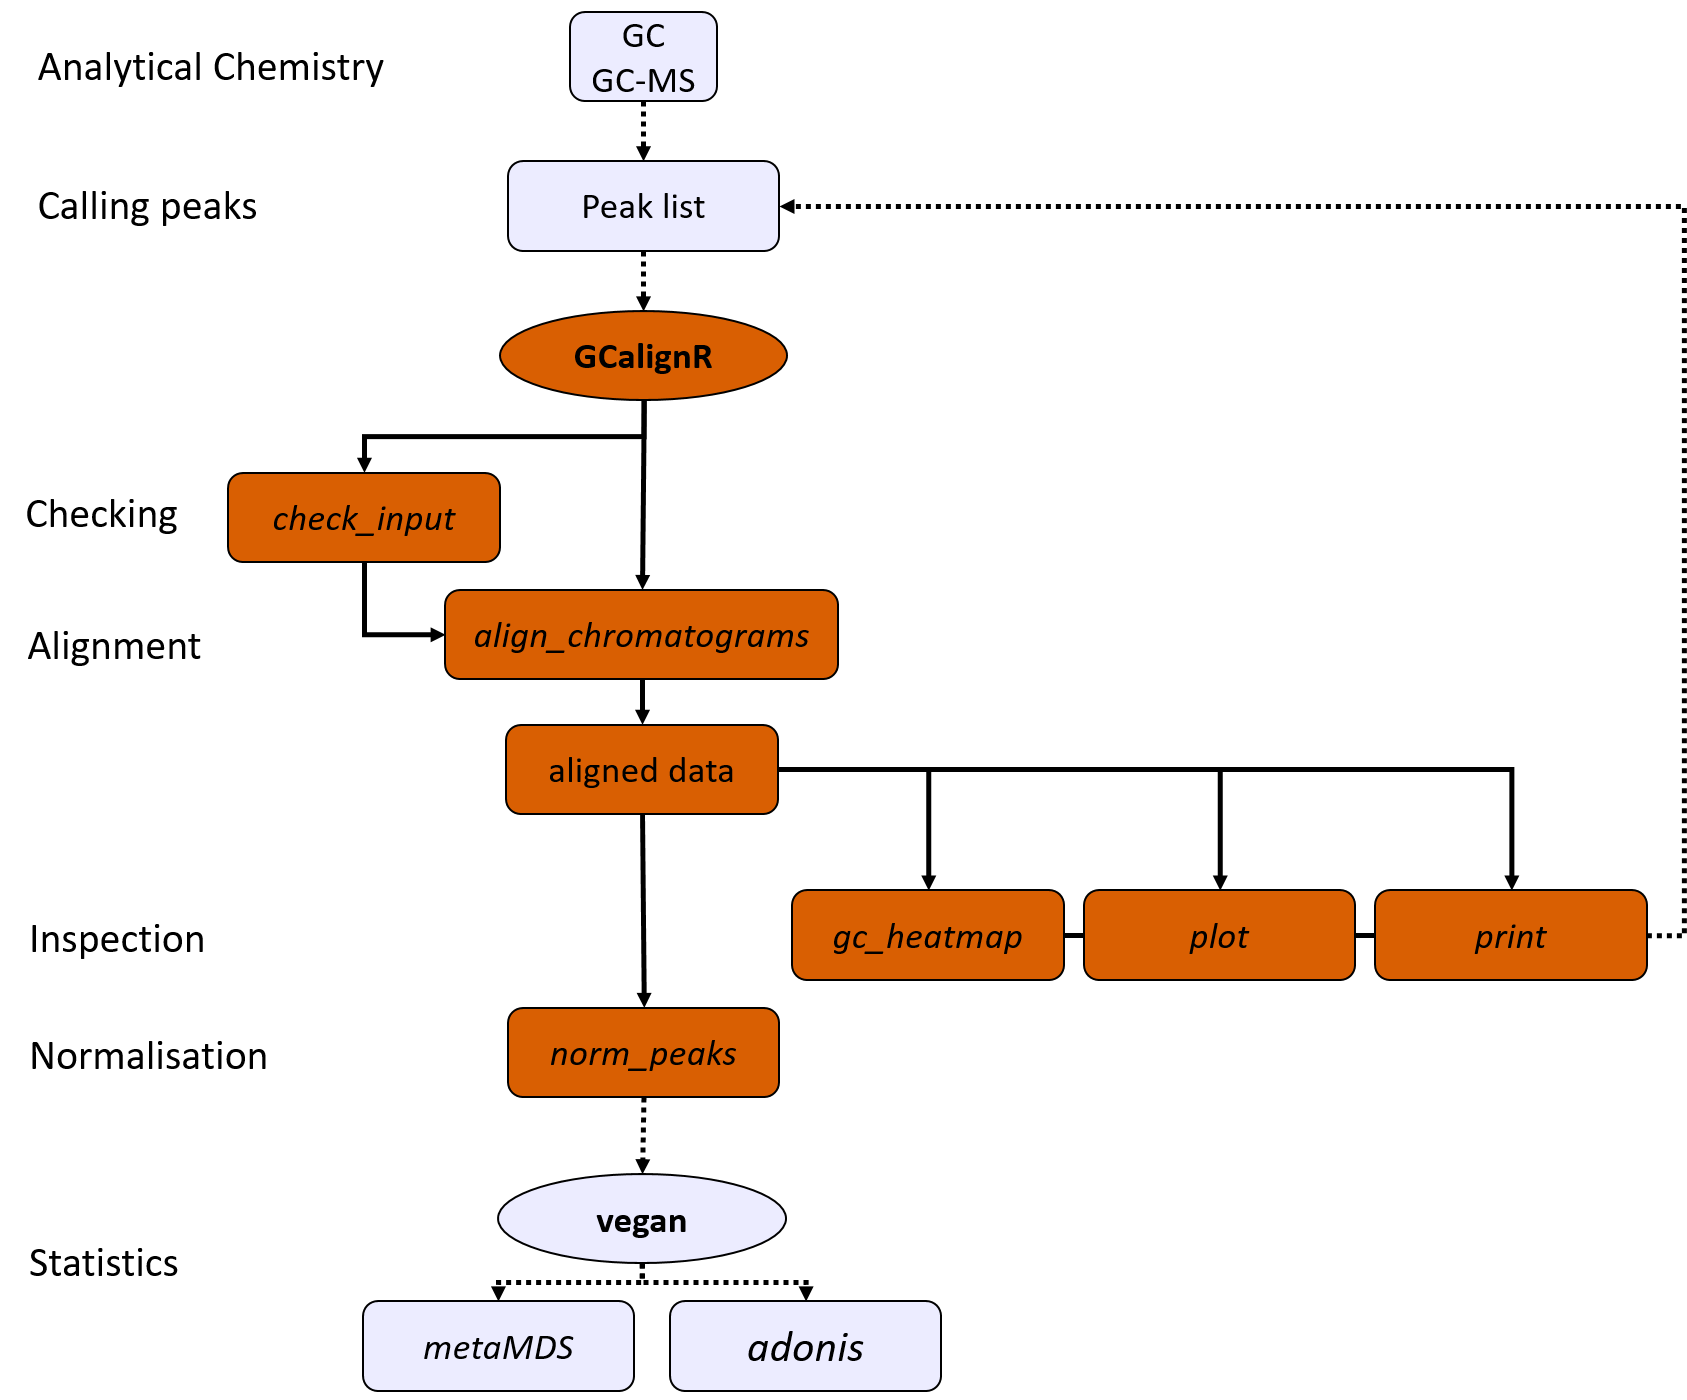
\includegraphics[width=13cm]{figures/workflow}
  \caption{\pkg{GCalignR} workflow. In addition to the alignment of substances across samples, the package provides functions for checking and inspecting the data. The aligned data is ready to use for analyses in conjunction with other packages.}
  \label{figure:workflow}
\end{figure}

\subsection{Example datasets}
For demonstration purposes \pkg{GCalignR} includes data of previously published chemical signatures that were obtained by sampling the skin of 82 Antarctic fur seals \textit{Arctocephalus gazella}. We showed that these signatures encode the membership to a breeding colony \cite{Stoffel.2015}. These data are available as a \emph{List} with individual samples included as a \emph{data.frame}. Two variables are available that represent the required retention time ("time") and peak abundance ("area"). 

\begin{example}
library(GCalignR)
# Seal scent data
data("peak_data") 
# Data is organized in one list of data.frames
str(peak_data[1:2]) 
#> List of 2
#>  $ C3:'data.frame':	217 obs. of  2 variables:
#>   ..$ time: num [1:217] 4.53 4.55 4.62 4.68 4.71 4.79 4.83 4.87 5.01 5.14 ...
#>   ..$ area: num [1:217] 3331224 1462381 4834211 7754401 1267617 ...
#>  $ C2:'data.frame':	217 obs. of  2 variables:
#>   ..$ time: num [1:217] 4.52 4.55 4.57 4.67 4.69 4.73 4.75 4.8 4.83 4.85 ...
#>   ..$ area: num [1:217] 2695110 5926253 10406833 6805905 1672849 ...
\end{example}

The second data set is comprised of three bumble bee species \textit{Bombus bimaculatus}, \textit{B. ephippiatus} and \textit{B. flavifrons} where signatures have been obtained from cephalic labial gland secretions of 24, 20 and 11 individuals respectively \citep{Dellicour.2013}. Cephalic secretions haven been demonstrated to aid in species identification \citep{Meulemeester.2011}. These data are available in a text file (figure \ref{figure:text}) in the format of typical output from proprietary peak detection software (e.g. XCalibur, Thermofischer Scientific or Labsolution, Shimadzu). Here, the names of samples and variables are given in the first two rows, while the peak data is included from below with single matrices concatenated horizontally.
\begin{figure}[htbp]
  \centering
  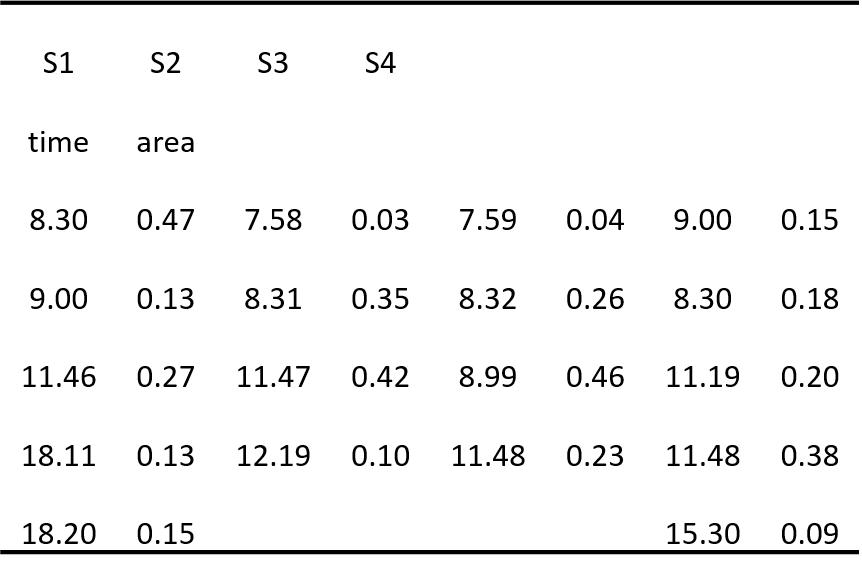
\includegraphics[width=8cm]{figures/text}
  \caption{Text files are the standard input of \pkg{GCalignR}}
  \label{figure:text}
\end{figure} 

\subsection{Checking the input}
The package provides the function \strong{check{\_}input} that enables the user to check the input for typical formatting errors and incomplete data. We encourage to use unique names for samples that should consist only of letters, numbers and underscores. If the data fails the test, indicative warnings are returned that guide in correcting these. Optionally, the argument \textit{list{\_}peaks} allows to create a barplot of the initial peak distribution to get an overview of the data:

\begin{example}
check_input(peak_data)
#> All checks passed!
#> Ready for processing with align_chromatograms
\end{example}

\section{Aligning substances among samples}
The alignment procedure is divided into five steps (figure \ref{figure:algorithm}). All steps are executed by the main function \textit{align{\_}chromatograms} and will be explained in in the next sections.
\subsubsection{Linear adjustments of chromatograms}
At first, chromatograms are linearly shifted with respect to a reference to account for systematic shifts in retention times among homologous chemicals shared by samples. Therefore, small linear adjustments are applied to the entire set of peaks in a chromatogram (figure \ref{figure:algorithm} A), such that the number of peaks that are shared at a threshold of two decimals (i.e. 0.6 seconds) is maximised.The parameter \textit{max{\_}linear{\_}shift} defines the maximum of linear shifts that are considered by the program. \newline
Note: This method relies on the occurrence of substances that are shared among most substances to produce efficient adjustments. If those are absent, it is unlikely to find a suitable shift and chromatograms remain untransformed. \par
A reference may be selected automatically by searching for the sample with the highest average similarity to all other samples based on the number of shared peaks prior to alignment. Alternatively, a chromatogram may be included that contains peaks of an internal standard which peaks are \textit{a-priori} known to occur in all samples. In this case, the sample should be named \code{"reference"} and will be removed after the alignment was conducted.

\newpage
\begin{figure}[htbp]
  \centering
  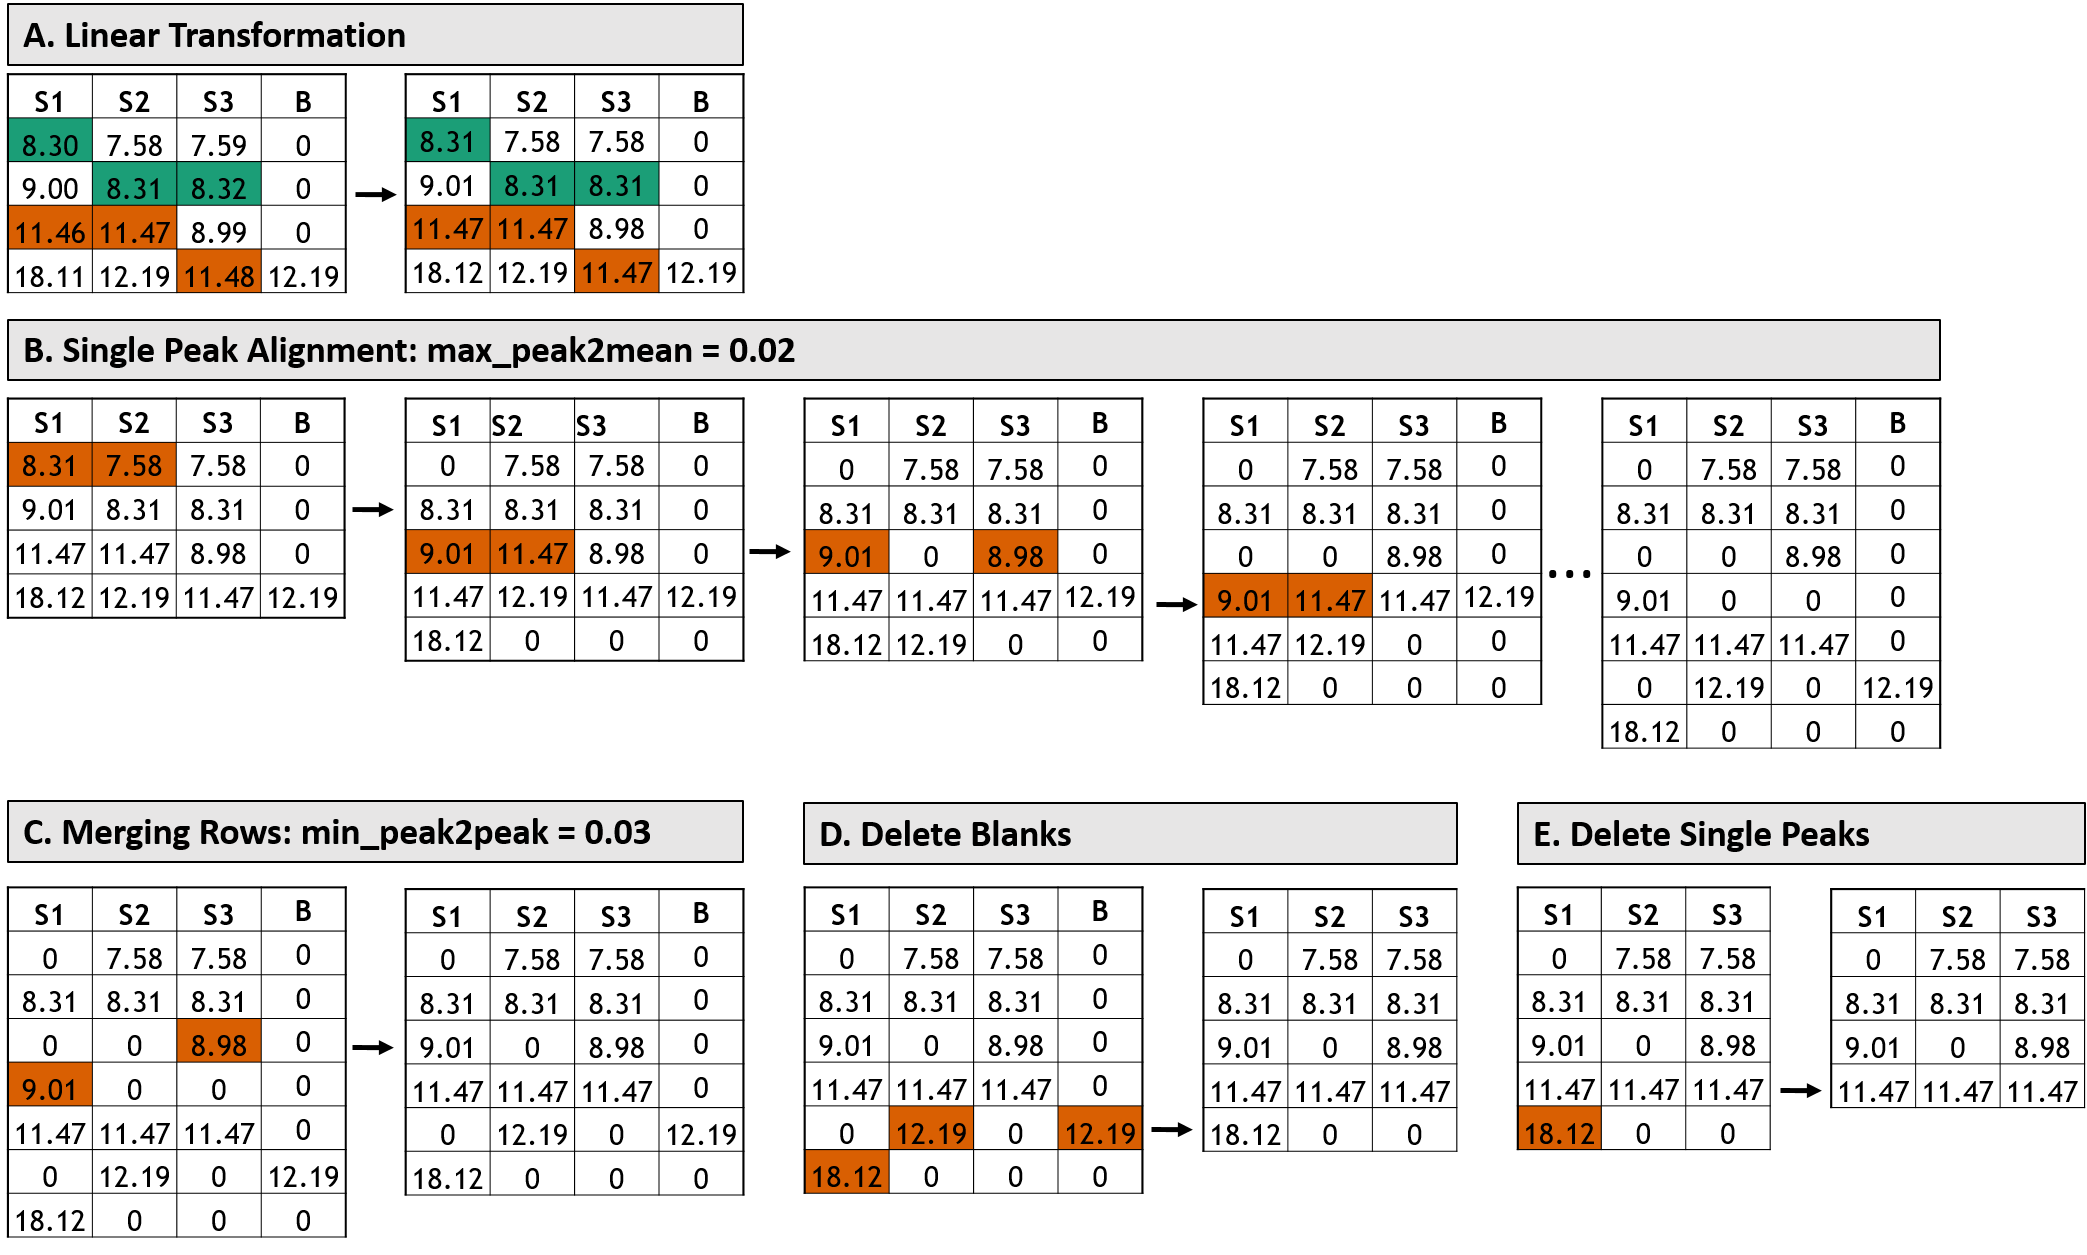
\includegraphics[width=13cm]{figures/algorithm}
  \caption{Overview of the algorithm performed by GCalignR. Row of matrices correspond to substances, columns are samples. Zeros indicate absence of peaks and are ignored in calculations. \strong{A}. Chromatograms are linearly shifted with respect to a reference (S2). Strong{B}. From left to right the first four steps from the input matrix to the final alignment are shown. Peaks are aligned row by row. Initially, always the second sample is compared to the first. Then the next sample is compared to all samples in previous columns until the last column is reached. Coloured cells represent conflicting retention times using \textit{max{\_}peak2mean = 0.02}. \strong{C}. After all peaks have been aligned, rows are merged depending on \textit{min{\_}peak2peak}, which defines the minimum difference that is expected between substances. If merging does not result in the loss of any data, rows are merged. \strong{D}. If specified, all peaks found in one or more blanks are removed as well as the blank itself. \strong{E}. Unique peaks which are present in only a single individual are not of interest for similarity analyses and can be removed as well.}
  \label{figure:algorithm}
\end{figure} 

\subsubsection{Piece-wise alignment of substances}
The core of the alignment procedure is based on clustering of individual peaks among samples. This is performed by examining retention times within single rows, where samples are compared consecutively with all previous samples starting with the second column (figure \ref{figure:algorithm} B):\par
If
\begin{equation}
rt_{m} > \left(\frac{\sum_{i=1}^{m-1}rt_{i}}{m-1}\right) + max{\_}peak2mean
\end{equation}
the examined peak is moved into the next row, whereas all previous samples are moved \par
if
\begin{equation}
rt_{m} < \left(\frac{\sum_{i=1}^{m-1}rt_{i}}{m-1}\right) - max{\_}peak2mean
\end{equation}  
with \textit{rt} = retention time; \textit{m} = current column and \textit{max{\_}peak2mean} defining the maximal deviation of the mean retention time.
\newline By considering the mean retention time among all previous samples the algorithm accounts for substance specific variations, such that less variable retention times are treated more stringent than chemicals exhibiting higher variability. Once the last retention time of a row was evaluated the whole procedure is repeated with the next row until the end of the retention time matrix was reached. Afterwards, rows with similar mean retention times are assessed for redundancy (figure \ref{figure:algorithm} C), which applies whenever a merging does not cause any loss of any information (i.e. no sample exists that contains substances in both rows). The similarity threshold is given by \textit{min{\_}peak2peak} defining the minimal difference between peaks that is expected.
\par In combination these two fairly simple algorithms align compounds by considering compound-specific variation in both steps.

\section{Workflow}
Here, we demonstrate the typical workflow using our seal data. This is done using the function \code{align{\_}chromatograms}. A list of all parameters and their description can be assessed from the documentation in the helpfile by typing \code{?align{\_}chromatograms}:

\begin{example}
seal_aligned <- align_chromatograms(data = peak_data,
                    conc_col_name = "area",
                    max_diff_peak2mean = 0.02,
                    min_diff_peak2peak = 0.05,
                    max_linear_shift = 0.05,
                    rt_col_name = "time",
                    delete_single_peak = T,
                    blanks = c("C2","C3"))
#> All checks passed!
#> Ready for processing with align_chromatograms
#> Run GCalignR
#> Start: 10:54:35
#>
#> Data for 84 samples loaded
#> A reference was not specified. Hence, 'P31' was selected on the basis of highest
#> average similarity to all samples (score = 37).
#> Start Linear Transformation with "P31" as a reference ... Done
#> Start Alignment of Peaks ...  This might take a while!
#> Iteration 1 out of 1  ... 
#> Merged Redundant Peaks
#> Peak Alignment Done 
#> Blank Peaks deleted & Blanks removed
#> Single Peaks deleted: 53 have been removed
#> 
#> Alignment was successful!
#> Time: 11:20:54
\end{example}

Now, we can inspect the results by retrieving summaries of the alignment process. The printing method summarises the function call including defaults that have not been explicitly specified during the function call. We also get the relevant information to retrace every step in the alignment:
\begin{example}
print(seal_aligned)
#>  Summary of Peak Alignment running align_chromatograms from package GCalignR
#>  Input: peak_data	Start:  2016-12-16 10:54:35 	Finished:  2016-12-16 11:20:54 
#>
#> Call:
#>  GCalignR::align_chromatograms(data=peak_data, conc_col_name=area,
#>  rt_col_name=time, max_diff_peak2mean=0.02, min_diff_peak2peak=0.05,
#>  blanks=(C2, C3), delete_single_peak=T, iterations=1, sep=\t,
#>  rt_cutoff_low=NULL, rt_cutoff_high=NULL, reference=NULL, max_linear_shift=0.05,
#>  merge_rare_peaks=FALSE)
#>
#> Summary of scored substances:
#>
#>   Peaks In_Blanks  Singular  Retained 
#>      506       167        53       286 
#>
#>  In total 506 substances were identified among all samples. 167 substances were
#>  present in blanks. The corresponding peaks as well as the blanks were removed
#>  from the data set. 53 substances were present in just one single sample and were
#>  removed. 286 substances are retained after all filtering steps.
#>
#> Sample Overview  The following 84 Samples were aligned to the reference 'P31':
#>  M2, M3, M4, M5, M6, M7, M8, M9, M10, M12, M14, M15, M16, M17, M18, M19, M20,
#>  M21, M23, M24, M25, M26, M27, M28, M29, M30, M31, M33, M35, M36, M37, M38, M39,
#>  M40, M41, M43, M44, M45, M46, M47, M48, P2, P3, P4, P5, P6, P7, P8, P9, P10,
#>  P12, P14, P15, P16, P17, P18, P19, P20, P21, P23, P24, P25, P26, P27, P28, P29,
#>  P30, P31, P33, P35, P36, P37, P38, P39, P40, P41, P43, P44, P45, P46, P47, P48
#>
#> For further details:
#>  Type 'gc_heatmap(seal_aligned)' to retrieve a heatmap for the alignment accuracy
#>  Type 'plot(seal_aligned)' to retrieve further diagnostic plots
\end{example}

The quality of an alignment will depend on sensible parameters that facilitate the (i) correction of linear shifts that might fall in a larger range with increasing sample size and (ii) and the variability of retention times. Optimally, linear shifts do not exhaust the range given by \code{max{\_}linear{\_}shift} completely, which would in turn indicate that not all uncertainties haven been fully compensated for. This can be assessed by some diagnostic plots:
\begin{example}
plot(seal_aligned)
\end{example}

\begin{figure}[htbp]
  \centering
  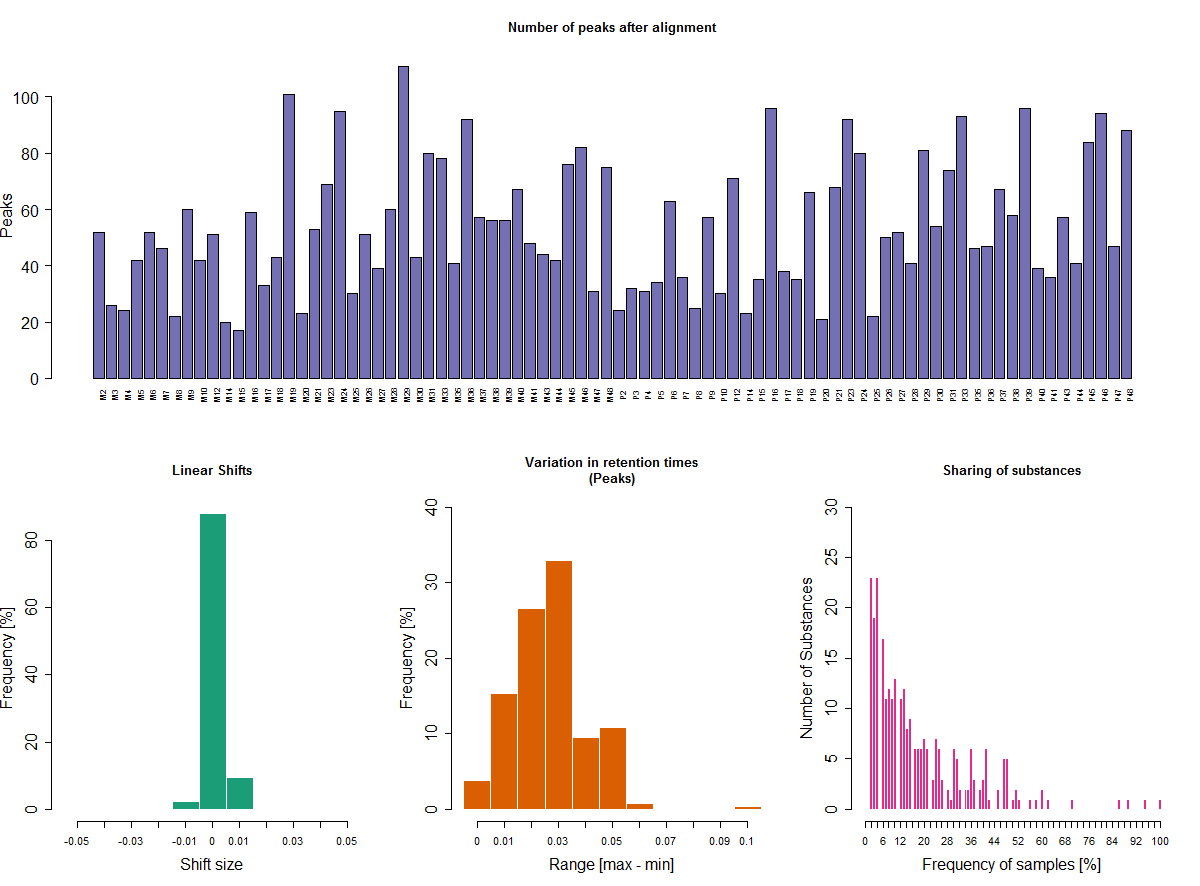
\includegraphics[width=13cm]{figures/plot-seal-aligned}
  \label{figure:plot_seal_aligned}
\end{figure} 


\bibliographystyle{plain}
\bibliography{ottensmann-stoffel-hoffman}

\address{Meinolf Ottensmann\\
  Department of Animal Behaviour\\
  Bielefeld University\\
   Morgenbreede 45\\
   33615 Bielefeld\\
  Germany\\}
\email{Meinolf.Ottensmann@web.de}

\address{Martin A. Stoffel\\
   Department of Animal Behaviour\\
  Bielefeld University\\
   Morgenbreede 45\\
   33615 Bielefeld\\
  Germany\\}
\email{Martin.Adam.Stoffel@gmail.com}

\address{Joseph I. Hoffman\\
  Department of Animal Behaviour\\
  Bielefeld University\\
   Morgenbreede 45\\
   33615 Bielefeld\\
  Germany\\}
\email{joseph.hoffman@uni-bielefeld.de}
